%!TEX root = ../../main.tex
\section{Projektgennemførelse}
\subsection{Specificering af projektet}
Katrines Kælder på Ingeniørhøjskolen Aarhus Universitet, havde lavet et projektforslag, om at de godt kunne tænkte at deres kasseapparat blev digitaliseret. Her var der beskrevet nogle fokuspunkter til produktet og givet en beskrivelse af hvad de forventede. Ud fra fokuspunkterne blev der udarbejdet nogle Use Cases så der kom en helt klar afgrænsning om hvad kasseapparatet skulle være i stand til når det er færdigt.
\newline
\newline
For at give en bedre inddeling og afgrænsning af kravene til produktet er der blevet brugt MoSCoW-metoden. Ved hjælp af denne er der blevet defineret funktionelle og ikke-funktionelle krav.  


\subsection{Arbejdsmetode}
Arbejdet med projektet er blevet udført iterativt og med SCRUM som inspirerende udviklingsproces. Inspireret af Scrum er projektforløbet blevet delt op i sprints, og gruppens arbejdsopgaver er blevet defineret på et scrumboard. 
\newline
Sprints blev i dette tilfælde valgt til at være to uger lange. Arbejdsopgaverne blev defineret på et Scrumboard, som projektgruppens medlemmer efterfølgende selv kunne påtage sig ansvaret for. Opgaverne blev rykket rundt på scrumboarded alt efter om de var fordelt, under arbejde, klar til review og færdig. 
\newline
\newline
Alle dele af projektet er blevet opdelt og lavet i små dele, dette gjorde det nemmere at overskue hvornår en opgave var færdig, men gjorde det også nemmere at arbejde parallelt på store opgaver. 

\begin{figure}[H]
	\centering
	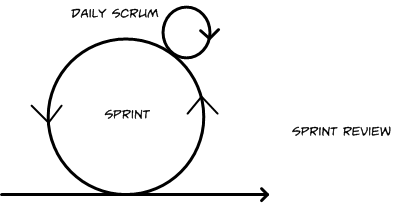
\includegraphics[scale=0.6]{Rapport/sprint_loop_events.PNG}
	\caption{sprint event}
	\label{fig:sprint}
\end{figure} 

\subsection{Proces}
Processen i dette semesterprojekt har været agil, og som nævnt tidligere, med Scrum som inspirerende udviklingsproces.
\newline
\newline
Flere gange om ugen blev der afholdt et dagligt scrum møde, hvor der er blevet talt om hvilke arbejdsopgaver der er blevet udført og hvilke der mangler. I starten af semesteret blev daily SCRUM udført ca. hver anden dag, mens der senere på semestret blev afholdt et møde hver dag. 


